\documentclass[openright, oneside]{gdutthesis}

\begin{document}

%%%%%%%%%%
% 生成封面
%%%%%%%%%%

\maketitle

\frontmatter % 正文前的摘要部分(罗马数字页码)

% 生成书脊
% \spine

%%%%%%%%%%
% 摘要
%%%%%%%%%%
\begin{abstract}{chinese}
\end{abstract}

\begin{abstract}{english}
\end{abstract}


%%%%%%%%%%
% 目录
%%%%%%%%%%

% 生成目录
\tableofcontents

%%%%%%%%%%
% 正文
%%%%%%%%%%

\mainmatter % 正文开始(阿拉伯数字页码)

% 诸论
\chapter{诸论}
\section{本题目的目的及意义}
\section{研究范围及要达到的技术要求}
\section{国内外的发展概况及存在的问题}
\section{本题目的指导思想及应解决的主要问题}


% 正文
\chapter{正文主体}
\section{问题的提出}
\section{研究工作的基本前提以及假设和条件}
\section{模型的建立以及实验方案的拟定}
\section{基本概念和理论基础}
\section{设计计算的主要方法和内容}
\section{实验方法实验内容及其分析}
\section{理论论证}
\section{理论在题目中的应用}
\section{题目得出的结果}
\section{对结果的讨论}

\chapter{\LaTeX 示例}
\section{公式}
\begin{equation}
\vec{P}_{i}(u)=\sum_{j=0}^{k} \vec{V}_{i} \Lambda_{i}\left(k ; \vec{\beta}_{1}, \cdots \vec{\beta}_{n} ; u\right)
\end{equation}

\begin{equation}
\frac{|A(s)|^{2}}{|A(o)|^{2}}=\frac{\rho_{1} \rho_{2}}{\left(s+\rho_{1}\right)\left(s+\rho_{2}\right)}
\end{equation}

\section{表格}

\begin{table}[h]
\centering
\caption{压降损失计算结果}
\label{table:jiangya}
\begin{tabularx}{\textwidth}{CCC}
\toprule[2pt]
换热器&热边压降损失&冷边压降损失\\
\midrule[1pt]
初级&2974.37&2931.52\\
次级&2924.65&3789.76\\
\bottomrule[2pt]
\end{tabularx}
\end{table}

\section{图}


\begin{figure}[!h]
\centering
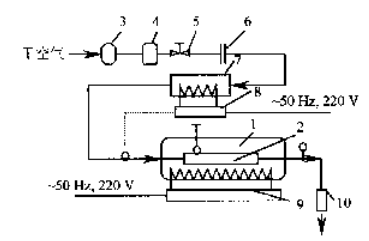
\includegraphics[width=0.5\textwidth]{figures/danguan}\\
\footnotesize
1-太阳模拟器;2-单管及 31 个 PCM 容器;3-气泵;\\
4-干燥过滤器;5-手动调节阀;6-孔板流量计;\\
7-空气预热器;8,9-调功器;10-空气换热器.\\
\caption{单管换热系统流程图}
\label{fig:danguan}
\end{figure}


\begin{figure}[!h]
  \subfigure[t][分布符合 $1 / f$ 规律图]{
    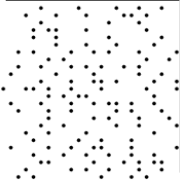
\includegraphics[width=0.25\textwidth]{figures/a}
  }
  \hfill
  \subfigure[t][大小与色彩符合 $1 / f$ 规律图]{
    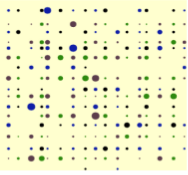
\includegraphics[width=0.25\textwidth]{figures/b}
  }
  \hfill
  \subfigure[t][间距、大小与色彩均符合 $1 / f$ 规律图]{
    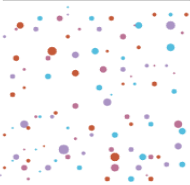
\includegraphics[width=0.25\textwidth]{figures/c}
  }
  \caption{图案例}
  \label{fig:tuan}
\end{figure}



%\input{tex/chapter2} % 可以按章分开各个文件
%...

% 结论
\chapter{结论}
\section{对所得结果与已有结果的比较}
\section{题目尚存在的问题}
\section{进一步开展研究的见解与建议}


\backmatter % 恢复奇数页开启新章

% 参考文献
\printbibliography[heading=bibintoc]

% 致谢
\begin{thanks}
\zhlipsum % 生成假文
\end{thanks}


\begin{appendix}
\appendixpage% 插入“附录”字样的分割页

\chapter{附录1标题}
\section{附录1节标题}

\chapter{附录2标题}

\end{appendix}


\end{document}
